\documentclass[serif,mathserif]{beamer}
\usepackage{amsmath, amsfonts, epsfig, xspace}
\usepackage{algorithm,algorithmic}
\usepackage{pstricks,pst-node}
\usepackage{multimedia}
\usepackage[normal,tight,center]{subfigure}
\setlength{\subfigcapskip}{-.5em}
\usepackage{beamerthemesplit}
\usetheme{keynote}
\usepackage{color}
%this is for the \hl{} highlight command 
\usepackage{soul}
%This makes it able to use different colours using \hlc[colourname]{}
\newcommand{\hlc}[2][yellow]{ {\sethlcolor{#1} \hl{#2}} }
%This is for framing text
\usepackage{framed}
\definecolor{shadecolor}{RGB}{255,127,0}

%----------Customize Title--
\defbeamertemplate*{title page}{customized}[1][]
{
  \begin{shaded}
  \usebeamerfont{title}\inserttitle\par
  \end{shaded}
  %\usebeamerfont{subtitle}\usebeamercolor[fg]{subtitle}\insertsubtitle\par
  %\bigskip
  %\usebeamerfont{author}\insertauthor\par
  %\usebeamerfont{institute}\insertinstitute\par
  %\usebeamerfont{date}\insertdate\par
  \usebeamercolor[fg]{titlegraphic}\inserttitlegraphic
}

%----------Beamer Modes---
%These modes are loaded with \mode<mode name>. They may
%also appear in the <overlay specification> option in the
%\begin{frame} command or as an option to the
%\documentclass.
%\modebeamer %(default)
%\modepresentation
%\modehandout
%\modetrans %(transparencies)
%\modearticle
%\modeall
%----------Print Handouts---
%To produce handouts, change the \documentclass command to
%\documentclass[handout]{beamer} and add
%\usepackage{pgfpages} This disables hyperlinks.
%\pgfpagesuselayout{4 on 1} Puts 4 slides on each page.
%\setbeamertemplate{navigation symbols}{} Turns on
%navigation bars at the bottom of each slide.
%----------Hacks-----------------
%http://www.shawnlankton.com/2008/02/beamer-and-latex-with-keynote-theme/
%\titlegraphic{\includegraphics[height=1cm]{iwmi}}
%\pgfdeclareimage[height=0.5cm]{iwmi}{iwmi}
%\logo{\pgfuseimage{iwmi}}
\setbeamercolor{titlelike}{parent=structure,fg=white}
%-----------------------------------

\title[AIT\hspace{2em}\insertframenumber/\inserttotalframenumber]{Planetary Surface RS}
%\author[Yann Chemin]{Yann Chemin }
%\institute{IWMI - U of Moratuwa}
%\date{} %leave out for today's date to be insterted

\begin{document}

{\usebackgroundtemplate{\includegraphics[height=\paperheight,width=\paperwidth]{PlanetarySurfaces}}
\begin{frame}[plain]
\titlepage
\end{frame}}

\Large

\transdissolve<5>

\begin{frame}
  \frametitle{Introduction}
\begin{table}
\begin{tabular}{lclc}
 BSc & 1995 & ISTOM & FR\\
 MSc & 1996 & Cranfield U. & UK\\
 DTSc & 2006 & AIT & TH\\
 PostDoc & 2008 & IRRI & PH\pause\\
 Senior Lecturer & 2009 & CSU & AU\pause\\
 Visiting Lecturer & 2011 & UoC & LK\pause\\
 Visiting Lecturer & 2012 & UoM & LK\pause\\
 Assoc. Prof. (eq.) & 2015 & UoM & LK\\
 \end{tabular}
\end{table}

\end{frame}

\transdissolve<5>

\begin{frame}
% \frametitle{Research summary}
\begin{center}
I worked most of my research life\\
\ \\
on evapotranspiration modeling\pause\\
\ \\
and its water management applications\pause\\
\ \\
in Asia and Australia
\end{center}
\end{frame}

\transdissolve<5>

\begin{frame}
 % \frametitle{of course}
  \centering
 {of course,}
  
\end{frame}

\transdissolve<5>

\begin{frame}
 % \frametitle{of course}
  \centering
{by remote sensing}
  
\end{frame}

\transdissolve<5>


{\usebackgroundtemplate{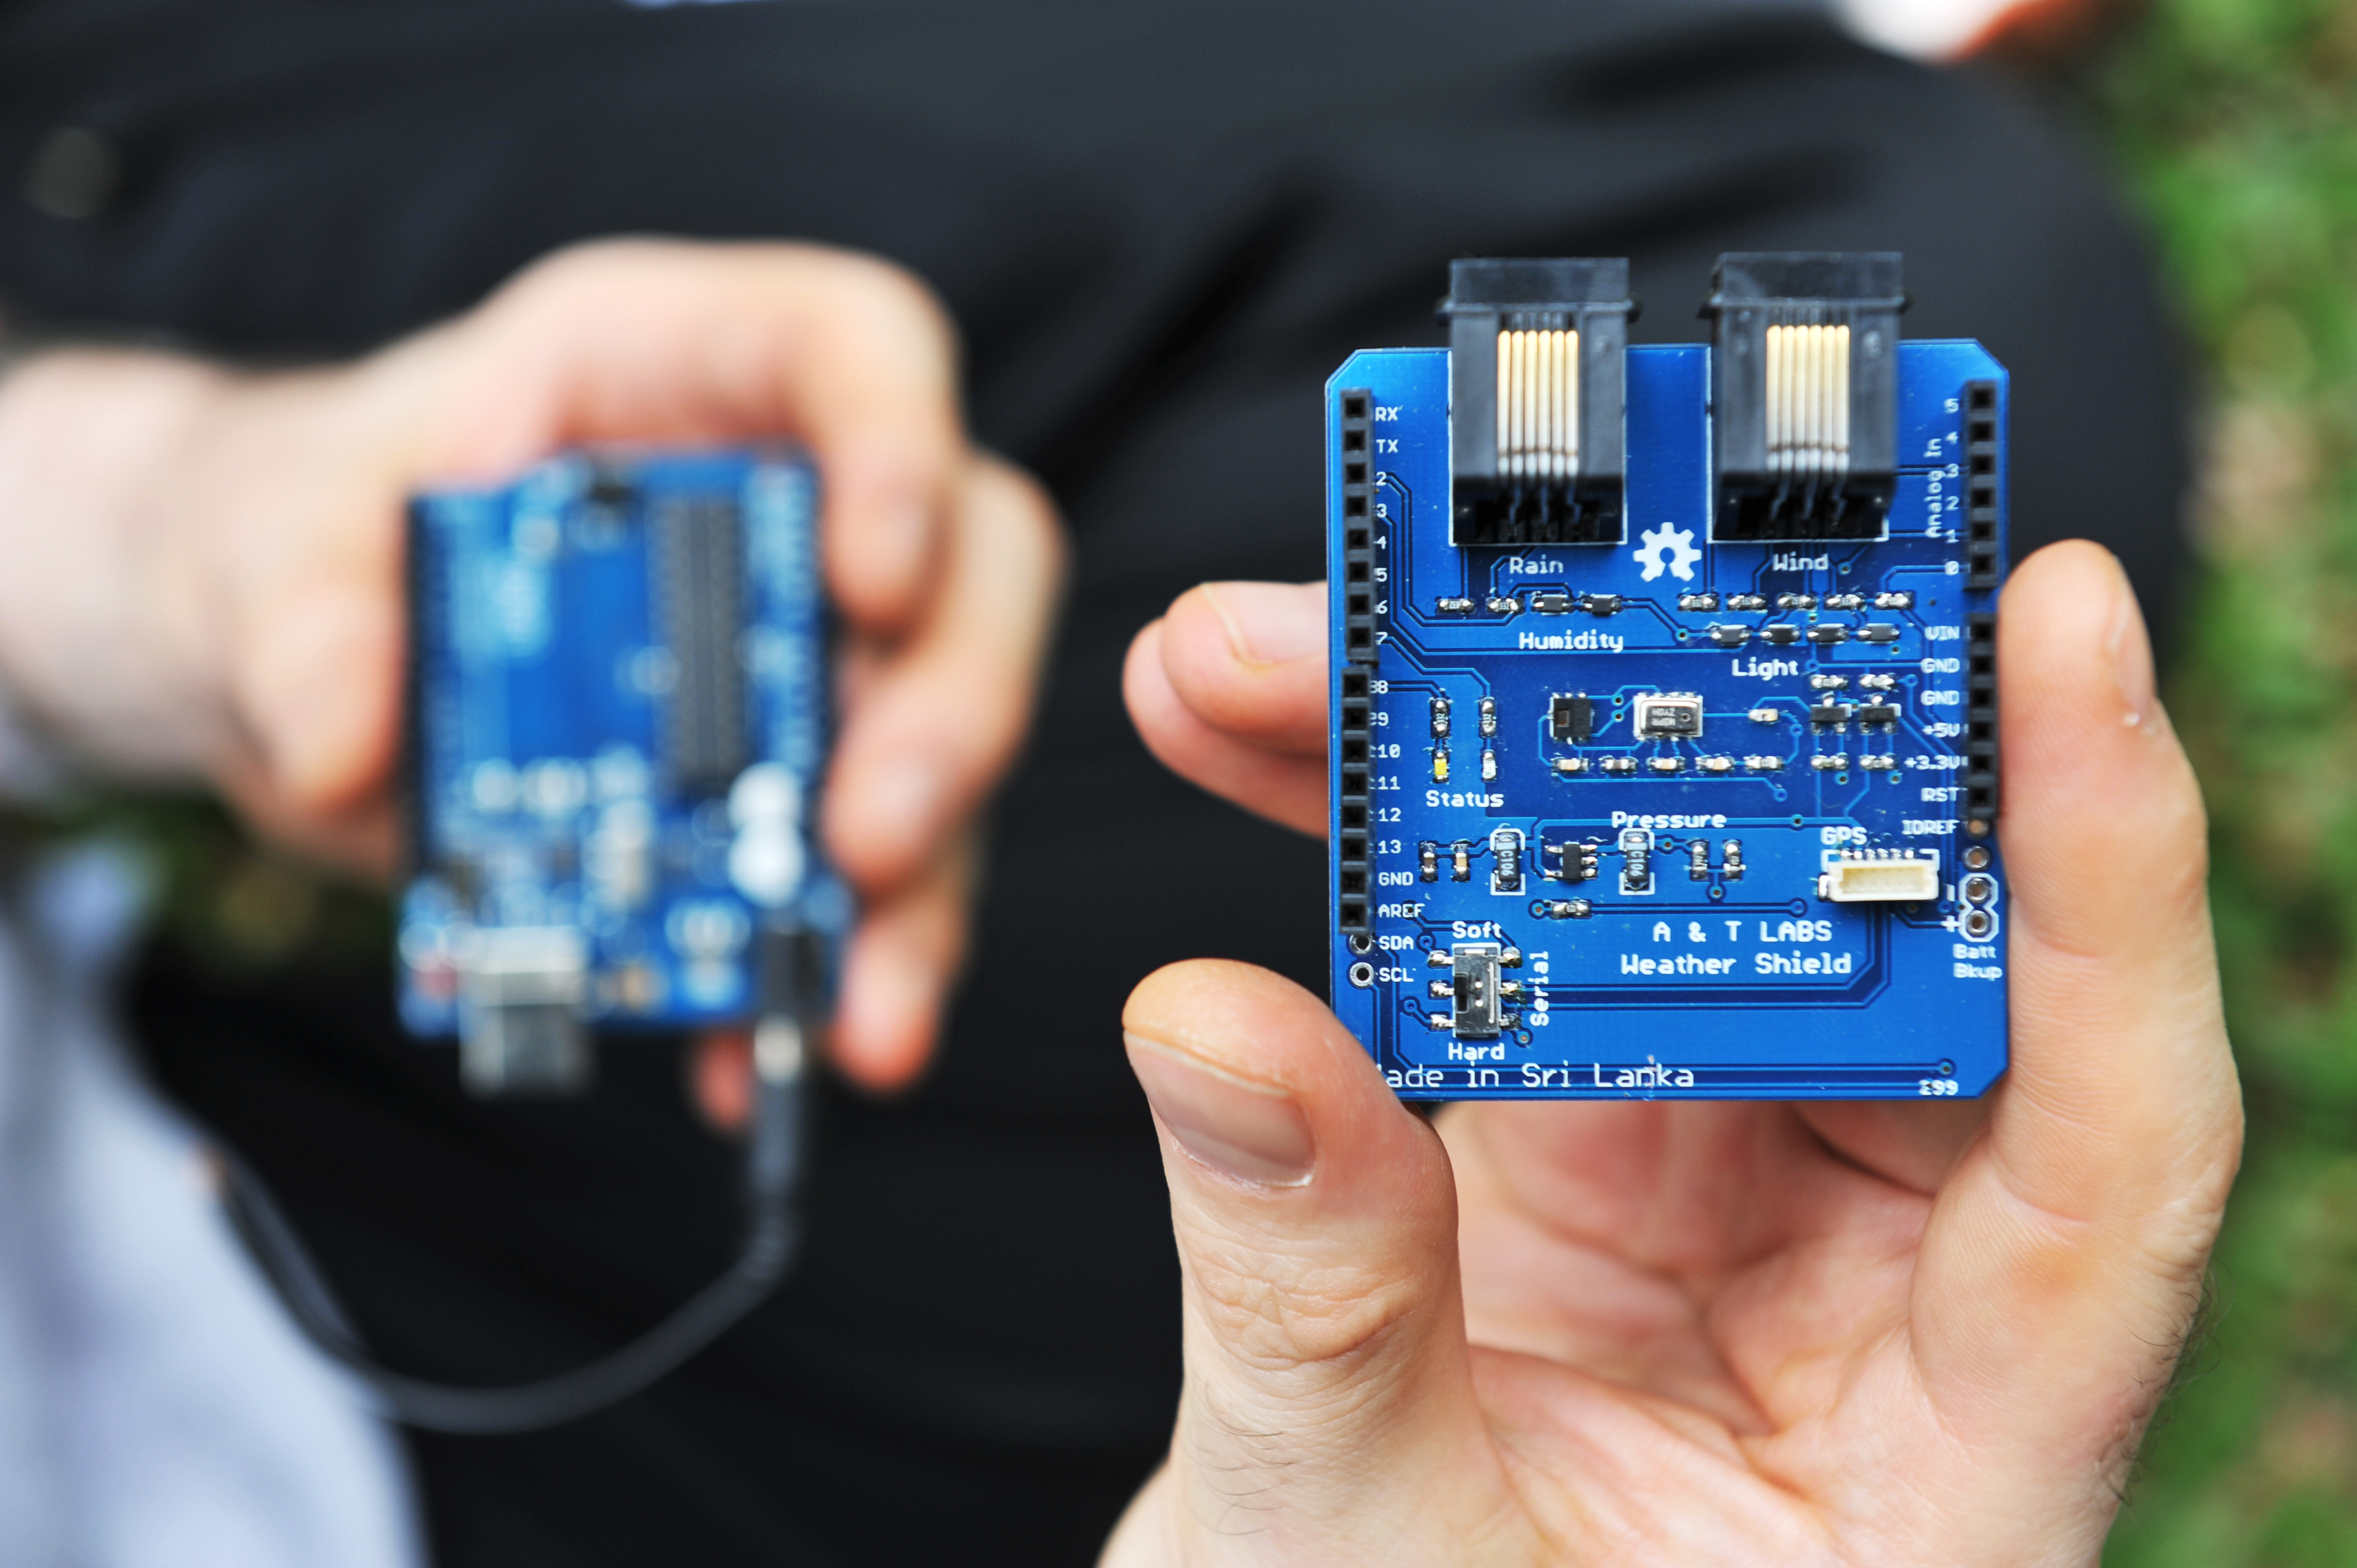
\includegraphics[height=\paperheight,width=\paperwidth]{fromNeil/Yann2.jpg}}
\begin{frame}[plain] %for empty slide
%\frametitle{Actual work}
\begin{shaded}
The National Climate Observatory
\end{shaded}
\end{frame}}

\transdissolve<5>

\begin{frame}
  \frametitle{A National Climate Observatory}
\begin{columns}
\column{0.6\textwidth}
\begin{center}
\begin{itemize}
 \item National grid of stations
 \item Land and sea
 \item Public website
 \item Mobile Apps
\end{itemize}
\end{center}

\column{0.4\textwidth}
\begin{center}
 \includegraphics[width=4.5cm]{ws500.png}
\end{center}
\end{columns}
\end{frame}

\transdissolve<5>

\begin{frame}
  \frametitle{National grid of stations}
\begin{columns}
\column{0.6\textwidth}
\begin{center}
\begin{itemize}
 \item 500 Weather Stations
 \item 5 minutes Reporting
 \item Climate-Based Grid
 \item Online
 \item 1/20$^{th}$ Cost 
 \item Improve Forecasting
\end{itemize}
\end{center}

\column{0.4\textwidth}
\begin{center}
 \includegraphics[width=4.5cm]{ws500.png}
\end{center}
\end{columns}
 \vspace{1mm}
\end{frame}

\transdissolve<5>

{\usebackgroundtemplate{\includegraphics[height=\paperheight,width=\paperwidth]{Lake_Argyle_wLVG}}
\begin{frame}[plain]
%\frametitle{Actual work}
\begin{shaded}
Water Level Virtual Gauge
\end{shaded}
\end{frame}}

\transdissolve<5>

\begin{frame}
  \frametitle{Water Level Virtual Gauge}
\begin{columns}
\column{0.45\textwidth}
\begin{center}
\begin{itemize}
 \item Landsat Imagery
 \item Water line
 \item 12cm V. accuracy
 \item 10-700Km2
 \item Next: \\Orbital Altimetry 
\end{itemize}
\end{center}

\column{0.5\textwidth}
\begin{center}
 \includegraphics[height=3cm]{IN_Maharana_Pratap_Sagar_wLVG1}
 %\includegraphics[height=2.5cm]{PK_TarbelaDam_wLVG1)\\
 %\includegraphics[height=3cm]{EG_AswanDam}
\end{center}
\end{columns}
\end{frame}

\transdissolve<5>

\begin{frame}
  \frametitle{water Level Virtual Gauge}
\begin{columns}
\column{0.5\textwidth}
\begin{center}
\includegraphics[height=2.5cm]{EG_AswanDam}\\
 \small{Aswan Dam (EG)}\\
 \vspace {2mm}
 \includegraphics[height=2.5cm]{PK_Mangla_wLVG1}\\
 \small{Mangla Dam (PK)}
\end{center}

\column{0.5\textwidth}
\begin{center}
 \includegraphics[height=2.5cm]{IN_Maharana_Pratap_Sagar_wLVG1}\\
 \small {Maharana Pratap Sagar (IN)}\\
 \vspace {2mm}
 \includegraphics[height=2.5cm]{PK_TarbelaDam_wLVG1}\\
 \small{Tarbela Dam (PK)}
\end{center}
\end{columns}
\end{frame}

\transdissolve<5>

{\usebackgroundtemplate{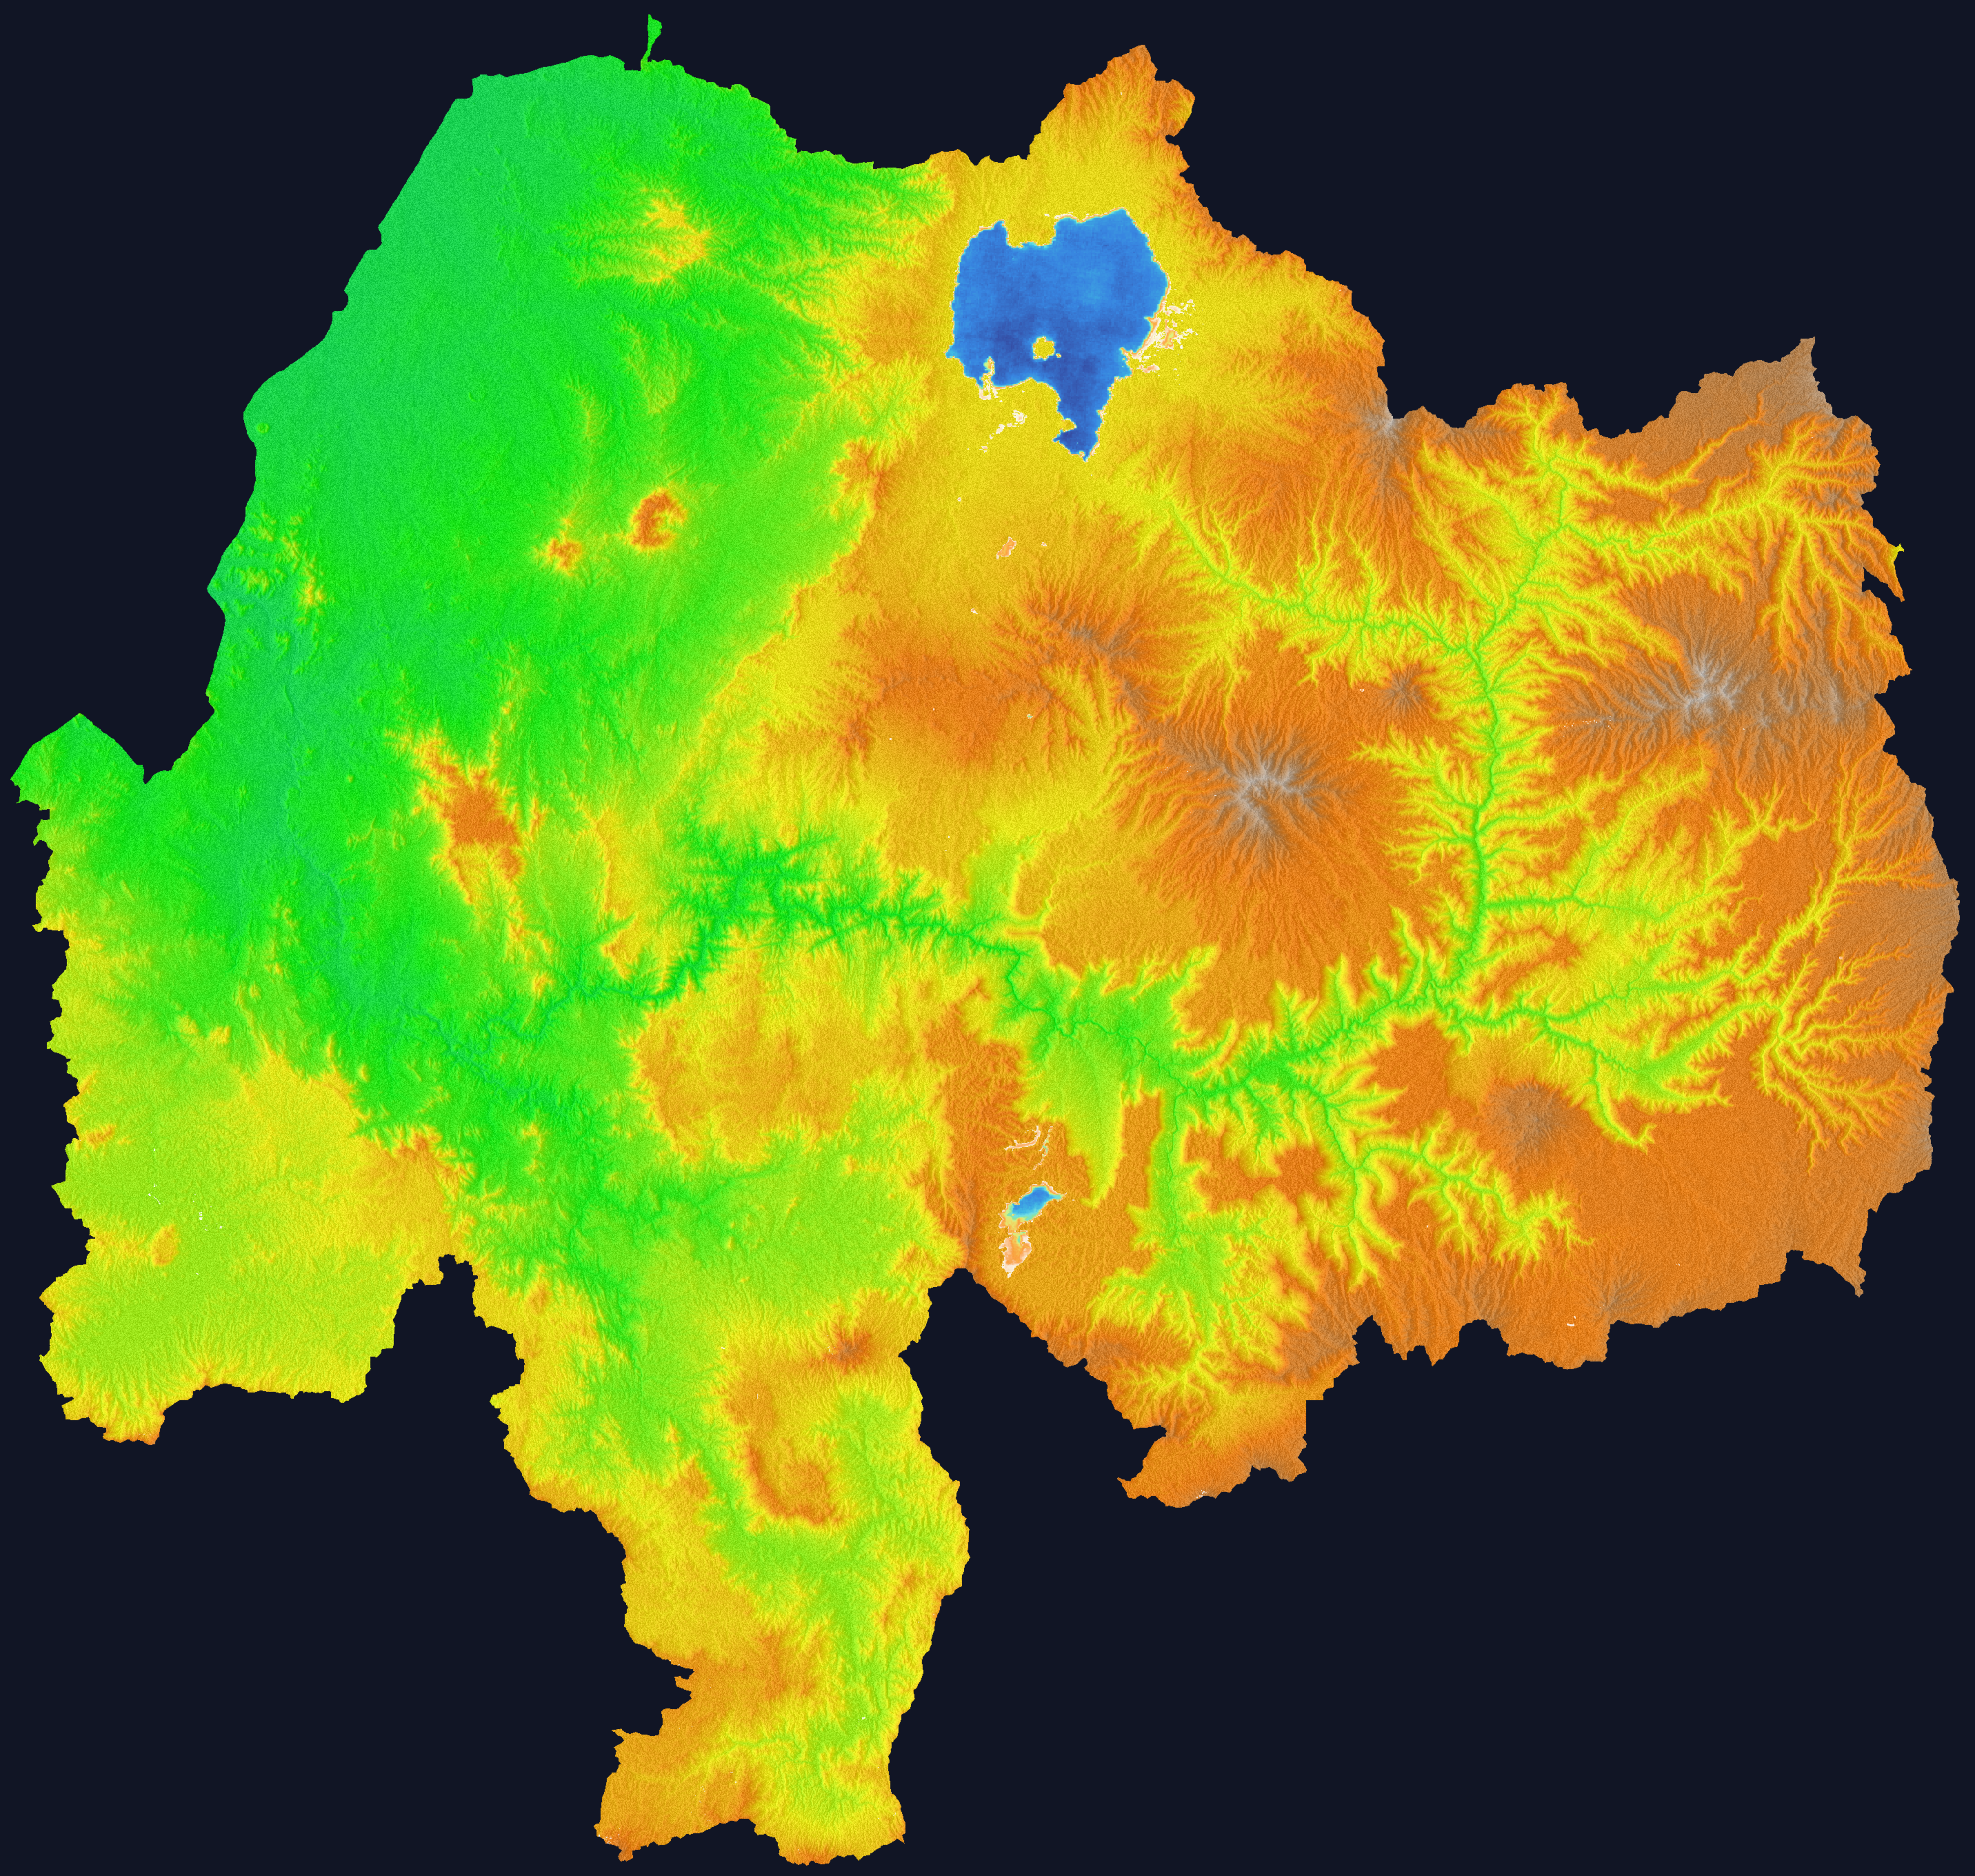
\includegraphics[height=\paperheight,width=\paperwidth]{WaterBorderEthUpperNile.pdf}}
\begin{frame}[plain]
%\frametitle{Actual work}
\begin{shaded}
Ethiopia Spring Maize
\end{shaded}
\end{frame}}

\transdissolve<5>

\begin{frame}
  \frametitle{Ethiopia Spring Maize}
\begin{columns}
\column{0.5\textwidth}
\begin{center}
\begin{itemize}
 \item Farmer perspective
 \item Water scarcity
 \item Spring Maize
 \item $\frac{1}{4}$ year is good
 \item Water Q missing?
\end{itemize}
\end{center}

\column{0.5\textwidth}
\begin{center}
 \includegraphics[width=5cm]{EthiopiaSpringMaize.png}
\end{center}
\end{columns}
\end{frame}

\transdissolve<5>

\begin{frame}
% \frametitle{Research summary}
\begin{center}
For the last 4 years\\
\ \\
while assuming my different employments\pause\\
\ \\
I am a DL BSc student in \\Planetary Sciences with Astronomy\pause\\
\ \\
University of London at Birkbeck\pause\\
\ \\
giving out my dissertation in April 2016
\end{center}
\end{frame}

\transdissolve<5>

{\usebackgroundtemplate{\includegraphics[height=\paperheight,width=\paperwidth]{A12}}
\begin{frame}[plain]
%\frametitle{Actual work}
\begin{shaded}
Hyperspectral Assessment of Apollo 12
\end{shaded}
\end{frame}}

\transdissolve<5>

\begin{frame}
  \frametitle{Apollo 12 landing site}
\begin{columns}
\column{0.5\textwidth}
\begin{center}
\begin{itemize}
 \item Push resolution
 \item Chandrayaan-1 M$^3$
 \item Hyperspectral
 \item Maybe Kaguya
 \item Connect with LSR
\end{itemize}
\end{center}

\column{0.5\textwidth}
\begin{center}
 \includegraphics[width=5cm]{Moon_A12_Medium_EM1_to_EM5.png}
\end{center}
\end{columns}
\end{frame}

\transdissolve<5>

{\usebackgroundtemplate{\includegraphics[height=\paperheight,width=\paperwidth]{Enceladus1}}
\begin{frame}[plain]
%\frametitle{Actual work}
\begin{shaded}
Hyperspectral Assessment\\ of Enceladus Brown Ice Deposits
\end{shaded}
\end{frame}}

\transdissolve<5>

\begin{frame}
  \frametitle{Enceladus brown ice deposits}
\begin{columns}
\column{0.5\textwidth}
\begin{center}
\begin{itemize}
 \item Cassini Probe
 \item Hyperspectral IR
 \item IDP? 
 \item High C dust: Vesta?
 \item Saturn E-ring?
 \item U of Milano
\end{itemize}
\end{center}

\column{0.5\textwidth}
\begin{center}
 \includegraphics[width=5cm]{Enceladus2}
\end{center}
\end{columns}
\end{frame}

\transdissolve<5>

{\usebackgroundtemplate{\includegraphics[height=\paperheight,width=\paperwidth]{KrakenMareT91}}
\begin{frame}[plain]
%\frametitle{Actual work}
\begin{shaded}
Titan Energy Balance
\end{shaded}
\end{frame}}

\transdissolve<5>

\begin{frame}
  \frametitle{Titan Energy Balance}
\begin{columns}
\column{0.5\textwidth}
\begin{center}
\begin{itemize}
 \item Cassini Probe
 \item IR VIMS Radar
 \item GCM constraints
 \item GCM for validation
 \item 2017 end of mission
 \item not another soon
 \item initial work only
\end{itemize}
\end{center}

\column{0.5\textwidth}
\begin{center}
 \includegraphics[width=5cm]{energybalance}
\end{center}
\end{columns}
\end{frame}

\transdissolve<5>

\begin{frame}
  \frametitle{Future}
  \begin{columns}
  \column{0.5\textwidth}
 \begin{center}
 \begin{itemize}
  \item Titan EB
  \item Magellan SAR PS
  \item SPICE Kernels API
  \item ISIS-GRASS part 2
 \end{itemize}
 \end{center}

 \column{0.5\textwidth}
 \begin{center}
  \includegraphics[width=5cm]{ISISGRASSCeres}
 \end{center}
 \end{columns}
\end{frame}

\transdissolve<5>

\begin{frame}
  \frametitle{Vision}
  \begin{columns}
  \column{0.5\textwidth}
 \begin{center}
 \begin{itemize}
  \item RS = Exploration
  \item Solar System varied
  \item Space RS varied
  \item Earth RS part of it
 \end{itemize}
 \end{center}

 \column{0.5\textwidth}
 \begin{center}
  \includegraphics[width=5cm]{PlanetarySurfaces}
 \end{center}
 \end{columns}
\end{frame}

\transdissolve<5>

%\begin{frame}
%  \frametitle{Equations}
%  Equations are easy
%  \begin{itemize}
%  \item Just copy and paste equations\pause
%  \item From the paper!
%    \begin{equation*}
%      \textbf{p}^* = \underset{\textbf{p}}{\arg\!\min}~\sum_{\textbf{x}}\left[ I(\textbf{W}(\textbf{x};\textbf{p})) - T(\textbf{x}) \right]^2
%    \end{equation*}
%  \end{itemize}
%\end{frame}
%
%\transdissolve<5>

%\begin{frame}
%  \frametitle{A Movie}
%  \begin{center}
%    \movie[height=5cm,width=6.5cm,poster,autostart,loop]{}{video1.avi}
%  \end{center}
%  \begin{itemize}
%  \item Movies only seem to work in Adobe Reader
%  \item Movie file is not embedded, it must be on the computer
%  \end{itemize}
%\end{frame}

\transdissolve<5>

\begin{frame}
  \frametitle{Questions}
\end{frame}
\end{document}
